\chapter{Efficiency of  Searching}
\label{CH:EFF:SEARCH}

Searching in a large database is a fundamental computational
task. Usually the information is partitioned into \defnfont{records}
and each record has a \defnfont{key} to use in the search. Suppose  we have a 
data structure $D$ of records. The search problem is as follows: given a search 
key $k$, either return the record associated with $k$ in $D$ (a 
\defnfont{successful search}), or indicate that $k$ is not found, without 
altering $D$ (an \defnfont{unsuccessful search}). If $k$ occurs more than once,
return any occurrence. The purpose of the search is usually to access data in 
the record (not merely the key). Simple examples are  searching a phone 
directory or a dictionary.

In this chapter we discuss searching in a general data structure as above. The 
more specialized problem of searching for a pattern in a text string is covered 
%later in Section~\ref{sec:strmatch}.
in the printed version of this textbook.

\section{The problem of searching}
\label{sec:search}

The most general data structure that allows searching is called an 
\emph{associative array},  \emph{table} or \emph{dictionary}.

In the general case, a key and a value are linked by \emph{association}.
An \defnfont{associative array} or \defnfont{dictionary} is an abstract 
data type relating a disjoint set of keys to an arbitrary set of values. Keys of
entries of an associative array may not have any ordering relation and may be
of unknown range. There is no upper bound on the size of this structure,
so that it can maintain an arbitrary number of different pieces of
information simultaneously. The analogy with a conventional word
dictionary may be misleading, because the latter has a lexicographical
order while dictionary structures need not be ordered.

Another name for this data type is \defnfont{table}. 
It takes its name from program compilation where
 a symbol table is used to record variables of a program, together with their
type, address, value, etc. Symbol table operations are also
fundamental to database systems.

\begin{Definition} The \defnfont{table} ADT is a set of ordered pairs 
(table entries) of the form \((k,v)\) where \(k\) is an unique \emph{key} and 
\(v\) is a data \emph{value} associated with the key \(k\). Each key uniquely
identifies its entry, and table entries are distinguished by keys
because no two distinct entries have identical keys. 

Basic operations defined for this structure are: construct (initialize) an 
empty table, enumerate table entries, search for an entry, insert, delete, retrieve, and 
update table entries.
\end{Definition}

Abstractly, a table is a mapping (function) from keys to values. Given a 
search key \(k\), \defnfont{table search} has to find the table entry 
\((k,v)\) containing that key. The found entry may be retrieved, or removed 
(deleted) from the table, or its value, \(v\), may be updated. If the table
has no such entry, a new entry with key \(k\) may be  created and inserted in 
the table. Operations on a table also initialize a table to the 
empty one or indicate that an entry with the given key is absent. Insertions 
and deletions modify the mapping of keys onto values specified by
the table.

\begin{Example}
\label{exm:adt:airports} 
Table~\ref{tab:adt-tbl} 
presents a very popular (at least in textbooks on algorithms and data
structures)  table having three-letter identifiers
of airports as keys and associated data such as
airport locations, as values. Each identifier
has a unique integer
representation \(k = 26^2 c_0 + 26c_1 + c_2\) where the \(c_i\); 
\(i=0,1,2\), are ordinal numbers of 
letters in the English alphabet
(A corresponds to  0, B to 1, \ldots, Z to 25). For example, 
AKL corresponds to $26^2 \cdot 0 + 26\cdot 10 + 11 = 271$. In total, there are  
$26^3=17576$ possible different keys and entries.
\end{Example}

\begin{table}[htb!]
\caption{\label{tab:adt-tbl}
A map between airport codes and locations.}
\centerline{
\begin{tabular}{|lr|lll|}\hline
\multicolumn{2}{|c|}{\textbf{Key}} &
\multicolumn{3}{c|}{\textbf{Associated value} \(v\)} 
\\ \hline
Code& \(k\) & City & Country & State / Place \\ \hline
AKL & 271 & Auckland    & New Zealand &                \\
DCA &2080 & Washington  & USA         & District of Columbia (D.C.) \\
FRA &3822 & Frankfurt   & Germany     & Hesse \\
GLA &4342 & Glasgow     & UK          & Scotland \\
HKG &4998 & Hong Kong   & China       &                \\
LAX &7459 & Los Angeles & USA         & California \\
SDF &12251& Louisville  & USA         & Kentucky  \\
ORY &9930 & Paris       & France      &              \\ \hline
\end{tabular}}
\end{table}

As can be seen from this example, we may map the keys to integers.

We deal with both \defnfont{static} (where the database is fixed in 
advance and no insertions, deletions or updates are done) and \defnfont{dynamic} 
(where insertions, deletions or updates are allowed) implementations of the table
ADT.

In all our implementations of the table ADT, we may simplify the analysis as follows. 
We use lists and trees as our basic containers. We treat each query or update of 
a list element or tree node, or comparison of two of them, as an elementary operation. 
The following lemma summarizes some obvious relationships.

\begin{Lemma}\label{lem:ss-us}
Suppose that a table is built up from empty by successive insertions, and we 
then search for a key $k$ uniformly at random. 
Let $T_{ss}(k)$ (respectively $T_{us}(k)$) be the time to 
perform successful (respectively unsuccessful) search for $k$. Then
\begin{itemize}
\item the time taken to retrieve, delete, or update an element with key $k$ is at least 
$T_{ss}(k)$; 
\item the time taken to insert an element with key $k$ is at least $T_{us}(k)$;
\item $T_{ss}(k) \leq T_{us}(k)$.
\end{itemize}

%\newpage
In addition
\begin{itemize}
\item
the worst case value for $T_{ss}(k)$ equals the worst case value for $T_{us}(k)$;
\item the average value of $T_{ss}(k)$ equals one plus the average of the 
times for the unsuccessful searches undertaken while building the table.
\end{itemize}
\end{Lemma}
\begin{proof}
To insert a new element, we first try to find where it would be if it were contained 
in the data structure, and then perform a single insert operation into the container. 
To delete an element, we first find it, and then perform a delete operation on the 
container. Analogous statements hold for updating and retrieval.
Thus for a given state of the table formed by insertions from an empty table, 
the time for successful search for a given element is the time that it took for 
unsuccessful search for that element, as we built the table, plus one. This means that 
the time for unsuccessful search is always at least the time for successful search 
for a given element (the same in the worst case), and the average time for 
successful search for an element in a table is the average of all the times for 
unsuccessful searches plus one. 
\end{proof}

If the data structure used to implement a table arranges the records in a list, 
the efficiency of searching depends on whether the list is sorted. In the case 
of the telephone book, we quickly find  the desired phone number (data record) 
by name (key). But it is almost hopeless to search directly for a phone number 
unless we have a special reverse directory where the phone number serves as a 
key. We discuss unsorted lists in the Exercises below, and sorted lists in the 
next section.


\subsection*{Exercises}

\begin{Exercise} \label{exr:seq-search}

The \defnfont{sequential search} algorithm 
simply starts at the head of a list and examines 
elements in order until it finds the desired key or reaches the end of the list. 
An array-based version is shown in Figure~\ref{seq-search}.

\begin{figure}[htb!]
\hspace*{1.2in}\begin{minipage}{5in}
\Algorithm{sequentialSearch}
{array $a[0..n-1]$; key $k$}
{index $i$ such that $a[i] = k$, or indicator ``not found''} 
{
\> \textbf{for} \(i\) $\leftarrow$ 0 \textbf{while} \(i < n\) 
                 \textbf{step} $i \leftarrow i+1$ \textbf{do}\\
\> \>\textbf{if} $a[i] = k$ 
              \textbf{then} \textbf{return} $i$ \\
\> \textbf{end for}\\
\> \textbf{return} \textsf{not found}\\
}
\end{minipage}
\caption{\label{seq-search} A sequential search algorithm.}
\end{figure}

Show that both successful and unsuccessful sequential  search in a list of size 
$n$ have worst-case and average-case time complexity $\Theta(n)$. 
\end{Exercise}

\begin{Exercise} \label{exr:seq-search-sorted}
Show that sequential search is slightly more efficient for sorted lists than 
unsorted ones. What is the time complexity of successful and unsuccessful search?
\end{Exercise}

\section{Sorted lists and binary search}\label{sec:bin:search}

A sorted list implementation allows for much better search method
that uses the divide-and-conquer paradigm. The basic idea of 
\defnfont{binary search} is simple. 
Let $k$ be the desired key for which we want to search.
\begin{itemize}
\item If the list is empty, return ``not found". Otherwise:
\item Choose the key $a[m]$ of the middle element of the list. If $a[m]=k$, return its record; 
if $a[m] > k$, make a recursive call on the head sublist;  if $a[m]<k$, make a 
recursive call on the tail sublist.
\end{itemize}

\begin{Example}
\label{eg:binsearch}
Figure~\ref{bsear-ex} illustrates binary search for
the key $k=42$ in a list of size 16. At the
first iteration, the search key 42 is compared to the 
key $a[7]  = 53$ in the middle position
$m=\lfloor (0+15)/2 \rfloor = 7$. 

\begin{figure}[htb!]
\centerline{
\illustr{bsear-ex.ps}{100mm}}
\caption{\label{bsear-ex} Binary search for the key 42.}
\end{figure}

Because $42 < 53$, the
second iteration explores the first half of the list
with positions $0,\ldots,6$. The search key is compared
to the key $a[3] = 33$ in the middle position
$m=\lfloor (0+6)/2 \rfloor = 3$. Because $42 > 33$, the
third iteration explores the second half of the current
sublist with positions $4,\ldots,6$. The comparison
to the key $a[5] = 49$ in the middle
position $m=\lfloor (4+6)/2 \rfloor = 5$ reduces the
search range to a single key, $a[4] = 42$,
because now $l = r = m = 4$. 
Because the single entry is equal to the search key, the
algorithm returns the answer 4.
\end{Example}


\subsection{Analysis of sorted list-based tables}
\label{sec:binsearch}

Binary search is readily seen to be correct by induction on the size of the list
(Exercise~\ref{exr:binary-search-correct}). 

The performance of binary search on an array is much better than on a linked list
because of the constant time access to a given element.

\begin{Lemma}
Consider a sorted list implementation of the table ADT.

Using an array, both successful and unsuccessful search take time in 
$\Theta(\log n)$, in both the average and worst case, as do retrieval and 
updating. Insertion and deletion take time in $\Theta(n)$ in the worst and 
average case.

Using a linked list, all the above operations take time in $\Theta(n)$. 
\end{Lemma}

\begin{proof}
Unsuccessful binary search takes $\lceil \lg (n+1)\rceil$ comparisons in 
every case, which is $\Theta(\log n)$. By Lemma~\ref{lem:ss-us}, 
successful search also takes time in $\Theta(\log n)$ on average and in the 
worst case. Insertion and deletion in arrays takes $\Theta(n)$ time on average 
and in the worst case.

For linked lists, the searches take time in $\Theta(n)$ and the list insertion 
and deletion take constant time.
\end{proof}

Binary search performs a predetermined sequence of comparisons
depending on the data size $n$ and the search key $k$. This sequence
is better analysed when a sorted list is represented as a 
\defnfont{binary search tree}. For simplicity of presentation, we suppress 
the data records and make all the keys integers. Background information on trees
is found in Section~\ref{sec:app:trees}.

\begin{Definition}
A \defnfont{binary search tree} (BST) is a binary tree that
satisfies the following ordering relation:
for every node $\nu$ in the tree, the values of all the keys
in the left subtree are smaller than (or equal, if duplicates allowed) 
to the key in $\nu$ and the  values of all the keys in the right 
subtree are greater than the key in $\nu$.
\end{Definition}

In line with the ordering relation, all the keys can be placed in sorted
order by traversing the tree in the following way: recursively visit,
for each node, its left subtree, the node itself, then its right subtree
(this is the so-called \defnfont{inorder} traversal). The relation is
not very desirable for duplicate keys; for exact data duplicates, we
should have one key and attach to it the number of duplicates.

The element in the middle position, $m_{0}=\lfloor (n-1)/2\rfloor$, of a
sorted array is the root of the tree representation.  The lower subrange,
$[0,\ldots,m_{0}-1]$, and the upper subrange, $[m_{0}+1,\ldots,n-1]$,
of indices are related to the left and right arcs from the root.
The elements in their middle positions, $m_{\mathrm{left},1}=\lfloor
(m_{0}-1)/2 \rfloor$ and $m_{\mathrm{right},1}=\lfloor (n + m_{0})/2
\rfloor$, become the left and right child of the root, respectively. This process 
is repeated until all the array elements are
related to the nodes of the tree. The middle element of each subarray
is the left child if its key is less than the parent key or the right
child otherwise.

\begin{figure}[htb!]
\centerline{
\illustr{btree-ex.ps}{100mm}}
\caption{\label{btree-ex} Binary tree representation of
a sorted array.}
\end{figure}
\begin{Example}
Figure~\ref{btree-ex}
shows a binary search tree for the 16 sorted keys in
Figure~\ref{bsear-ex}.
The key $a[7] =53$ is the root of
the tree. The lower $[0..6]$ and the upper $[8..15]$
subranges of the search produce the two children of the root:
the left child $a[3] =33$ and the right child
$a[11] =81$. All other nodes are built similarly.
\end{Example}

The tree representation interprets binary search
as a pass through the tree from the root to a desired key.
If a leaf is reached but the key is not found, then the search
is unsuccessful. The number of comparisons to find a key 
is equal to the number of nodes along the unique path from the root to
the key (the depth of the node, plus one).

A static binary search always yields a tree that is well-balanced:
for each node in the tree, the left and right subtrees have height that differs 
by at most $1$. Thus all leaves are on at most two levels. This property is used 
to define AVL trees in Section~\ref{sec:balanced}.


\subsection{Implementation of binary search}

Algorithm \algfont{binarySearch} in Figure~\ref{bin-search} 
searches for key \(k\) in a sorted array $a$.

\begin{figure}[htb]
\hspace*{.7in}\begin{minipage}{5in}
\Algorithm{binarySearch}
{array $a[0..n-1]$; key $k$}
{index $i$ such that $a[i] = k$, or indicator ``not found''}
{
\> $l \leftarrow 0$; $r\leftarrow n-1$\\
\> \textbf{while} $l \le r$ \textbf{do}\\ 
\> \>$m\leftarrow\lfloor(l+r)/2\rfloor$\\
\> \>\textbf{if} $a[m] < k$
             \textbf{then} $l \leftarrow m+1$\\
\> \>\textbf{else} \textbf{if} $a[m] > k$ 
             \textbf{then} $r\leftarrow m-1$
             \textbf{else} \textbf{return} $m$\\
\> \>\textbf{end if}\\
\> \textbf{end while}\\
\> \textbf{return} \textsf{not found}\\
}
\end{minipage}
\caption{\label{bin-search} Binary search with three-way comparisons.}
\end{figure}

The search starts from the whole
array from $l=0$ to $r=n-1$. If \(l\) and \(r\) ever
cross, $l > r$, then the desired
key is absent, indicating an unsuccessful search. Otherwise,
the middle position of the odd range or rounded down
``almost middle'' position  of 
the even one, $m=\left\lfloor\frac{l+r}{2}\right\rfloor$,  is computed.
The search key, $k$, is compared to the key $a[m]$ in this position:

\begin{itemize}
 \item If $k = a[m]$,
then return the found position $m$.
 \item If $k < a[m]$, then the key may be
in the range $l$ to $m-1$ so that $r\leftarrow m-1$ at next step. 
 \item If $k > a[m]$, then it
may be in the range $m+1$ to $r$ so that $l\leftarrow m+1$ at next step. 
\end{itemize}

Binary search is slightly accelerated if the test for a successful
search is removed from the inner loop in Figure~\ref{bin-search} and the
search range is reduced by one in all cases. To determine whether
the key $k$ is present or absent, a single test is performed outside the
loop (see Figure~\ref{fast-bin-search}). If the search key $k$ is not
larger than the key $a[m]$ in the middle position $m$, then it may be in
the range from $l$ to $m$. The algorithm breaks the while-loop when the
range is 1, that is, $l = r$, and then tests whether there is a match.

\begin{figure}[htb!]
\hspace*{1.3in}\begin{minipage}{5in}
\Algorithm{binarySearch2}
{array $a[0..n-1]$; key $k$}
{index $i$ such that $a[i] = k$, or indicator ``not found''}
{
\> $l \leftarrow 0$; $r\leftarrow n-1$\\
\> \textbf{while} $l < r$ \textbf{do}\\ 
\> \>$m\leftarrow\lfloor(l + r)/2\rfloor$\\
\> \>\textbf{if} $a[m] < k$
               \textbf{then} $l\leftarrow m+1$\\
\> \>\textbf{else} $r \leftarrow m$\\
\> \textbf{end while}\\
\> \textbf{if} $a[l] = k$ \textbf{then} 
                \textbf{return} $l$ \\
\> \textbf{else} \textbf{return} \textsf{not found} \\
}
\end{minipage}
\caption{\label{fast-bin-search} Faster binary search with two-way
comparisons.}
\end{figure}

\subsection*{Exercises}

\begin{Exercise}
\label{ex:binsearch}
Perform a search for the key $41$ in the situation of 
Example~\ref{eg:binsearch}.
\end{Exercise}

\begin{Exercise}\label{exr:binsearch:comp}
How many comparisons will binary search make in the
worst case to find a key in a sorted array of size \(n=10^6\)?
\end{Exercise}

\begin{Exercise}\label{exr:binary-search-correct}
Prove that both given array implementations of binary search correctly find an 
element or report that it is absent.
\end{Exercise}

\begin{Exercise}\label{exr:interpol-search-bad}
If we have more information about a sorted list, \defnfont{interpolation search} 
can be (but is not always) much faster than binary search. It is the method 
used when searching a telephone 
book: to find a name starting with ``C" we open the book not in the middle, but 
closer to the beginning. 

To search for an element between position $l$ and $r$ with $l < r$, we choose 
\(\rho = \frac{ k - a[l]}{a[r] - a[l]}\)
and the next guess is  
\(
m = l + 
\left \lceil \rho (r - l) \right \rceil.
\)

Give an example of a sorted input array of $8$ distinct integers 
for which interpolation search performs no better than sequential search.
\end{Exercise}

\begin{Exercise}\label{exr:interpol:search}
Determine how many positions interpolation search will
examine to find the key \(85\) among the ten keys 
\((10,20,35,45,55,60,75,80,85,100)\).
\end{Exercise}

\section{Binary search trees}
\label{bin-search-tree}

In Section~\ref{sec:binsearch} we have already used a binary search
tree to specify sequences of comparisons and simplify the performance
analysis of binary search. Now we use a binary search tree not just as a mathematical 
object to aid our analysis, but as an explicit data structure that implements the 
table ADT. 

\begin{figure}[htb!]
\centerline{
\illustr{btree-e1.ps}{80mm}}
\caption{\label{btree-e1} Binary trees: only the leftmost tree is
a binary search tree.}
\end{figure}
\begin{Example}
In Figure~\ref{btree-e1}, two trees are not binary search trees 
because the key $2$ in the middle tree is
in the right subtree of the key $3$, 
and the keys $11$ and $12$ in the rightmost tree are
in the left subtree of the key $10$.
\end{Example}
Binary search trees implement efficiently the basic search, insert, and remove
operations of the table ADT. In addition a BST allows for more operations 
such as sorting records by their keys, finding the minimum key, etc (see Exercises).

Binary search trees are more complex than heaps. Only a root or 
leaves are added to or removed from a heap, whereas
any node of a binary search tree may be removed.

\begin{figure}[htbp]
\centerline{
\illustr{findinsr.ps}{70mm}}
\caption{\label{findinsr} Search and insertion in the binary search tree.}
\end{figure}

The search operation resembles usual binary search in that it starts 
at the root and moves either left or right along the tree, depending on 
the result of comparing the search key to the key in the node. 

\begin{Example}
\label{exm:find:a}
To find key $\textsf{8}$ in the leftmost tree in
Figure~\ref{btree-e1}, we
start at the root $10$ and go left because $\textsf{8} < 10$. This move
takes us to $3$, so we turn right (because $\textsf{8} > 3$) to $5$. Then we
go right again ($\textsf{8} > 5$) and encounter $8$. 
\end{Example}

\begin{Example}
\label{exm:find:b}
To find key $7$, we repeat the same path. But, when we are at node $8$, we 
cannot turn left because there is no such link. Hence, $7$ is not found. 
\end{Example}

Figure~\ref{findinsr} illustrates both Examples~\ref{exm:find:a} and
\ref{exm:find:b}. It shows that the node with key $7$ can be inserted
just at the point at which the unsuccessful search terminates.  

The removal operation is the most complex because removing a node may
disconnect the tree. Reattachment must retain the ordering condition but
should not needlessly increase the tree height. The standard method of removing 
a node is as follows.
\begin{itemize}
\item A leaf node is simply deleted. 
\item An internal node with only one child
is deleted after its child is linked to its parent node.
\item If the node has two children, then it should be swapped with the node 
having the smallest key in its right subtree. 
The latter node is easily found (see Exercise~\ref{exr:bst-min-max-med}). After 
swapping, the node can be removed as in the previous cases, since it is now in 
a position where it has at most one child. 
\end{itemize}

This approach appears asymmetric but various modifications do not really
improve it. The operation is illustrated in Figure~\ref{btr-dele}.

\begin{figure}[htb!]
\centerline{
\illustr{btr-dele.ps}{80mm}
}
\caption{\label{btr-dele} Removal of the node with key $10$ from
the binary search tree.}
\end{figure}

\subsection{Analysis of BST-based tables}

\begin{Lemma}
The search, retrieval, update, insert and remove operations in a BST 
all take time in $O(h)$ in the worst case, where $h$ is the height of the tree. 
\end{Lemma}
\begin{proof}
The running time of these operations is proportional to the 
number of nodes visited. For the find and insert operations, this equals 
$1$ plus the depth of the node, but for the remove operation it equals the 
depth of the node plus at most the height of the node. In each case this is 
$O(h)$. 
\end{proof}

For a well-balanced tree, all operations take logarithmic time. The problem is 
that insertions and deletions may destroy the balance, and in practice BSTs 
may be heavily unbalanced as in Figure~\ref{btr-bala}. So in the worst case the 
search time is linear, $\Theta(n)$, and we have an inferior form of sequential search 
(because of the extra overhead in creating the tree arcs).

Figure~\ref{btr-4b} presents all variants of inserting the four 
keys $1$, $2$, $3$, and $4$ into an empty binary search tree. Because only 
relative ordering is important, this corresponds to any four keys 
\((a[i]: i=1,\ldots,4)\) such that
\(
a[1] < a[2] < a[3] < a[4]
\).

\begin{figure}[htb!]
\centerline{
\illustr{btr-4a.ps}{120mm}}
\centerline{
\illustr{btr-4b.ps}{80mm}}
\caption{\label{btr-4b} Binary search trees obtained by
permutations of $1,2,3,4$.}
\end{figure}

There are in total $4!=24$ possible insertion orders given in
Figure~\ref{btr-4b}.
Some trees result from several different insertion sequences, and more balanced 
trees appear more frequently than unbalanced ones.


\begin{Definition}
The \defnfont{total internal path length}, 
\(S_\tau(n)\), of a binary tree $\tau$  is the sum of the 
depths of all its nodes. 
\end{Definition}

The average node depth, \(\frac{1}{n}S_{\tau}(n)\),
gives the average time complexity of a successful search in a
particular tree $\tau$. The average-case time complexity of searching
is obtained by averaging the total internal path lengths for all the trees of 
size \(n\), that is, for all possible \(n!\) insertion orders, assuming that 
these latter occur with equal probability, \(\frac{1}{n!}\). 


\begin{Lemma}\label{lem:bst:ave}
Suppose that a BST is created by $n$ random insertions starting from an empty tree.
Then the expected time for successful and unsuccessful search is 
$\Theta(\log n)$. The same is true for update, retrieval, insertion and deletion.
\end{Lemma}

\begin{proof}
Let $S(n)$ denote the average of $S_\tau$ over all insertion 
sequences, each sequence considered as equally likely. 
We need to prove that $S(n)$ is $\Theta(n \log n)$. 

It is obvious that $S(1)=0$. Furthermore, any $n$-node tree,
$n > 1$, contains a left subtree with $i$ nodes, a root at height $0$,
and a right subtree with $(n-i-1)$ nodes where $0 \le i \le n-1$,
each value of $i$ being by assumption equiprobable. 

For a fixed $i$, $S(i)$ is the average total internal path length in the
left subtree with respect to its own root and $S(n-i-1)$ is the
analogous total path length in the right subtree. The root of the tree
adds $1$ to the path length of each other node. Because there are
$n-1$ such nodes, the following recurrence holds:
\(S(n) = (n-1) + S(i) + S(n-i-1)\) for \(0 \le i \le n-1\).
After summing these recurrences for all $i=0,\ldots,n-1$ and averaging,
just the same recurrence as for the average-case 
quicksort analysis (see Lemma~\ref{lem:qsort:ave:comp}) is obtained:
\(
S(n) = (n-1) + \frac{2}{n} \sum_{i=0}^{n-1} S(i) 
\).
Therefore, the average total internal path length is $\Theta(n \log n)$. The 
expected depth of a node is therefore in $\Theta(\log n)$. This means that 
search, update, retrieval and insertion take time in $\Theta(\log n)$. The same 
result is true for deletion (this requires the result that the expected height 
of a random BST is $\Theta(\log n)$, which is harder to prove---see Notes).
\end{proof}

Thus in practice, for random input, all BST operations take time about 
$\Theta(\log n)$. However the worst-case linear time complexity, $\Theta(n)$, 
is totally unsuitable in many applications, and deletions can also destroy 
balance. 

We tried to eliminate the worst-case degradation of 
quicksort by choosing a pivot that performs well on random input data
and relying on the very low probability of the worst case. Fortunately, binary 
search trees allow for a special general technique, called \defnfont{balancing}, 
that guarantees that the worst cases simply cannot occur. Balancing 
restructures each tree after inserting new nodes in such a way as to prevent 
the tree height from growing too much. We discuss this more in 
Section~\ref{sec:balanced}.

\begin{figure}[htb!]
\centerline{
\illustr{btr-blns.ps}{60mm}}
\caption{\label{btr-blns} Binary search trees of height about $\log n$.}
\end{figure}

\begin{figure}[htb!]
\centerline{
\illustr{btr-bala.ps}{60mm}}
\caption{\label{btr-bala} Binary search trees of height about $n$.}
\end{figure}


\subsection{Implementation of BST}

A concrete implementation of a BST requires explicit links between nodes, each 
of which contains a data record, and is more complicated than the other 
implementations so far. A programming language that supports easy manipulation of
objects makes the coding easier. We do not present any (pseudo)code in this book.

\subsection*{Exercises}

\begin{Exercise}\label{exr:bst-min-max-med}
Show how to find the maximum (minimum) key in a binary search tree. What is the 
running time of your algorithm? How could you find the median, or an arbitrary 
order statistic?
\end{Exercise}

\begin{Exercise} \label{bst-dist}
Suppose that we insert the elements $1,2,3,4,5$ into an initially 
empty BST. If we do this in all 120 possible orders, which trees occur most often? 
Which tree shapes (in other words, ignore the keys) occur most often?
\end{Exercise}

\begin{Exercise} \label{exr:bst-extreme}

Suppose that we insert the elements $1,2,3,4$ in some order into an initially 
empty BST. Which insertion orders yield a tree of maximum height? Which yield a 
tree of minimum height?  
\end{Exercise}

\begin{Exercise}\label{exr:bst-sort}
Show how to output all records in ascending order of their keys, given a BST. 
What is the running time of your algorithm? 
\end{Exercise}

\section{Self-balancing binary and multiway search trees}
\label{sec:balanced}

Because balanced binary search trees are more complex than the standard
ones, the insertion and removal operations usually take
longer time on the average. But because of the resulting balanced structure,
the worst-case complexity is $O(\log n)$. In
other words, the total internal path lengths of the trees are fairly close to
the optimal value.

\subsection{AVL, red-black, and AA-trees}
\label{ss:avl}

\begin{Definition}
An \defnfont{AVL tree} is a binary search tree 
with the additional
balance property that, for any node in the tree, the heights of
the left and right subtrees can differ by at most $1$. 
\end{Definition}

This balance condition ensures height $\Theta(\log n)$
for an AVL tree despite being less restrictive than requiring the tree to be 
complete. Complete binary trees have too rigid  a balance condition 
which is difficult to maintain when new nodes are inserted.

\begin{Lemma}
The height of an AVL tree with $n$ nodes is $\Theta(\log n)$.
\end{Lemma}
\begin{proof}

Due to the possibly different heights of its subtrees, an
AVL tree of height $h$ may contain fewer than $2^{h+1}-1$ nodes.
We will show that it contains at least $c^{h}$ nodes for some constant $c>1$, 
so that the maximum height of a tree with $n$ items is $\log_{c}n$.

Let $S_{h}$ be the size of the smallest AVL tree of height $h$. It is
obvious that $S_{0}=1$ (the root only) and $S_{1}=2$ (the root and one
child). The smallest AVL tree of height $h$ has subtrees of height $h-1$
and $h-2$, because at least one subtree is of height $h-1$ and the second
height can differ at most by $1$ due to the AVL balance condition. These
subtrees must also be the smallest AVL trees for their height, so that $S_{h}=
S_{h-1}+S_{h-2}+1$. 

By mathematical induction, we show easily that
$S_{h}=F_{h+3}-1$  where $F_{i}$ is the $i$-th Fibonacci number
(see Example~\ref{ex:fibonacci:formula})
because $S_{0} = F_{3}-1$, $S_{1} = F_{4}-1$, and $S_{i+1}=
(F_{i+3}-1)+(F_{i+2}-1)+1 \equiv F_{i+4}-1$. Therefore, 
for each AVL tree with $n$ nodes
\(
n \ge S_{h} \approx \frac{\phi^{h+3}}{\sqrt{5}} - 1
\)
where $\phi \approx 1.618$. Thus, 
the height of an AVL tree with $n$ nodes satisfies
the following condition:
\(
h \le 1.44 \cdot \lg (n+1) - 1.33
\),
and the worst-case height is at most 44\% more than the minimum height for
binary trees. 
\end{proof}

Note that AVL trees need in the worst case only about 44\% more comparisons than
complete binary trees. They behave even better in the average case. 
Although theoretical estimates are unknown, the average-case height of a
randomly constructed AVL tree is close to $\lg n$. 

All basic operations in an AVL tree have logarithmic worst-case running time. 
The difficulty is, of course, that simple BST insertions and deletions can 
destroy the AVL balance condition. We need an efficient way to restore the 
balance condition when necessary. All self-balancing binary search trees use 
the idea of \defnfont{rotation} to do this.

\begin{Example}\label{ex:rotation}
Figure~\ref{fig:treerotation} shows a left rotation at the node labelled $p$ and 
a right rotation at the node labelled $q$ (the labels are not related to the 
keys stored in the BST, which are not shown here). These rotations are mutually 
inverse operations. Each rotation involves only local changes to the tree, 
and only a constant number of pointers must be updated, independent of the tree 
size. If, for example, there is a subtree of large height below $a$, then the 
right rotation will decrease the overall tree height.

\begin{figure}[htb]
\begin{center}
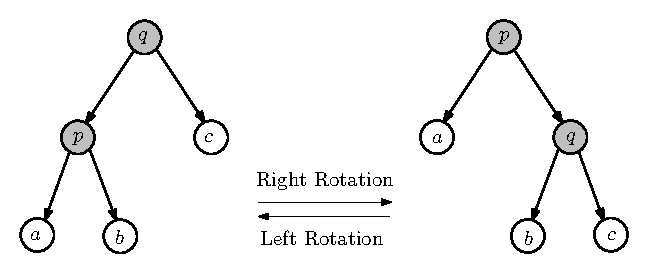
\includegraphics[width=6cm]{figs/treerotation}
\caption{\label{fig:treerotation}Left and right rotations of a BST.}
\end{center}
\end{figure}

\end{Example}

The precise details of exactly when a rotation is required, and which kind, 
differ depending on the type of balanced BST. In each case the programming of
the insertion and removal operations is quite complex, as is the analysis. 
We will not go into more details here---the reader should consult the  
recommended references.

Balancing of AVL trees requires extra memory and heavy
computations. This is why even more relaxed efficient balanced search
trees such as red-black trees are more often used in practice.

\begin{Definition}
A \defnfont{red-black tree} is a binary search tree such that 
every node is coloured either red or black, and every non-leaf node 
has two children. In addition, it satisfies the following properties: 
\begin{itemize}
\item the root is black;
\item all children of a red node must be black;
\item every path from the root node to a leaf must contain the same number of 
black nodes.
\end{itemize}
\end{Definition}

\begin{Theorem}
If every path from the root to a leaf contains $b$ black 
nodes, then the tree contains at least $2^{b}-1$ black nodes.
\end{Theorem}
\begin{proof}

The statement holds for $b=1$ (in this case
the tree contains either the black root only or the black
root and one or two red children). In line with the induction hypothesis, 
let the statement hold for all red-black trees with $b$ black nodes  in every 
path. If a tree contains $b+1$ black nodes in every path and has two black 
children of the root, then the tree contains two subtrees with $b$ black nodes 
just under the root and has in total at least 1+$2 \cdot(2^{b}-1) = 2^{b+1}-1$ 
black nodes. If the root has a red child, the latter has only black children, 
so that the total number of the black nodes can become even larger. 
\end{proof}

Each path cannot contain two consecutive red nodes and increase more
than twice after all the red nodes are inserted. Therefore, the height
of a red-black tree is at most $2\lceil \lg n \rceil$, and the
search in it is logarithmic, $O(\log n)$.

Red-black trees allow for a very fast search. This data structure has
still no precise analysis of its average-case performance. Its
properties are found either experimentally or by analysing red-black
trees containing random $n$ keys. There are about $\lg n$ comparisons per search 
on the average and fewer than $2\lg n + 2$ comparisons in the
worst case. Restoring the tree after insertion or deletion of single node 
requires $O(1)$ rotations and $O(\log n)$ colour changes in the worst case.

Another variety of balanced tree, the \defnfont{AA-tree}, becomes more efficient 
than a red-black tree when node deletions are frequent. An AA-tree has 
only one extra condition with respect to a red-black tree, namely that 
the left child may not be red. This property simplifies the removal 
operation considerably.

\subsection{Balanced B-trees: efficiency of external search}
\label{ss:B-tree}

The B-tree is a popular
structure for ordered databases in external memory such as magnetic or
optical disks. The previous ``Big-Oh'' analysis is invalid here because
it assumes all elementary operations have equal time complexity. This
does not hold for disk input / output where one disk access corresponds
to hundreds of thousands of computer instructions and the number of
accesses dominates running time. For a large database of many millions
of records, even logarithmic worst-case performance of red-black or
AA-trees is unacceptable. Each search should involve a very small number
of disk accesses, say, 3--4, even at the expense of reasonably
complex computations (which will still take only a small fraction of a disk access time).

Binary tree search cannot solve the problem because even 
an optimal tree has height $\lg n$. To decrease the
height, each node must have more branches. The height of an
optimal $m$-ary search tree ($m$-way branching) is roughly
$\log_{m} n$ (see Table~\ref{tbl:m-ary:branch}), or  
$\lg m$ times smaller than with an optimal binary tree 
(for example, $6.6$ times for $m=100$).

\begin{table}[htb!]
\caption{\label{tbl:m-ary:branch}Height of the optimal $m$-ary 
search tree with $n$ nodes.}
\centerline{
\begin{tabular}{|c|r|r|r|r|r|} \hline 
$n$ & $10^{5}$ & $10^{6}$ & $10^{7}$ & $10^{8}$  & $10^{9}$ \\ \hline
$\lceil \log_{2}n \rceil$  & 17  & 20  & 24  & 27  & 30 \\ \hline 
$\lceil \log_{10}n \rceil$ & 5   & 6   & 7   & 8   & 9 \\ \hline 
$\lceil \log_{100}n \rceil$ & 3   & 3   & 4   & 4   & 5 \\ \hline
$\lceil \log_{1000}n \rceil$ & 2   & 2   & 3   & 3   & 3 \\ \hline
\end{tabular}}
\end{table}

\begin{figure}[htb]
\begin{center}
\illustr{mtr-ex.ps}{90mm}
\caption{\label{mtr-ex} Multiway search tree of order $m=4$.}
\end{center}
\end{figure}

Figure~\ref{mtr-ex} shows that the search and the traversal of a
multiway search tree generalize in a straightforward way the binary
search tree operations. If in the latter case the search key is compared
to a single key in a node in order to choose one of two branches or stop
in the node, in an $m$-ary tree, the search key is compared to at most
$m-1$ keys in a node to choose one of $m$ branches. The major difference
is that multiple data records are now associated only with leaves
although some multiway trees do not strictly follow this condition. Thus
the worst-case and the average-case search involve the tree height and
the average leaf height, respectively.

\begin{Example}
Search for a desired key $k$ in Figure~\ref{mtr-ex} is guided by
thresholds, for example at the root it goes left if $k<4$, down if $4
\le k < 10$, and right if $k \ge 10$. The analogous comparisons are
repeated at every node until the record with the key $k$ is found at a
leaf or its absence is detected. Let $k=17$. First, the search goes
right from the root (as $17 > 10$), then goes to the third child of the
right internal node (as $17 \le 17 < 20$), and finally finds the desired
record in that leaf.
\end{Example}

\begin{Definition}
A \defnfont{B-tree} of order $m$ is an $m$-ary tree such that:
\begin{itemize} 
\item the root is either a leaf or it has between $2$ and
$m$ children inclusive; 
\item each nonleaf node (except possibly the root) has
between $\lceil m/2 \rceil$ and $m$ children inclusive;
\item each nonleaf node with $\mu$ children has $\mu-1$
keys, $(\theta[i]: i=1,\ldots,\mu-1)$, to guide the search where $\theta[i]$ is the smallest key in subtree $i+1$;
\item all leaves are at the same depth;
\item data items are stored in leaves, each storing between $\lceil l/2 \rceil$ and $l$ items, for some $l$.
\end{itemize} 
\end{Definition}

Other definitions of B-trees (mostly with minor changes) also exist, but
the above one is most popular. The first three conditions specify the
memory space each node needs (first of all, for $m$ links and $m-1$
keys) and ensure that more than half of it, except possibly in the root,
will be used. The last two conditions form a well-balanced tree.

\begin{figure}[htb]
\begin{center}
\illustr{mtr-b4.ps}{90mm}
\caption[2--4 B-tree with the leaf storage size 7.]%
{2--4 B-tree with the leaf storage size 7
($2..4$ children per node and $4..7$ data items per leaf).}
\label{mtr-b4} 
\end{center}
\end{figure}

\begin{note}
B-trees are usually named by their \defnfont{branching limits}, 
that is, $\lceil m/2 \rceil$--$m$, so that $2$--$3$ and $6$--$11$ 
trees are B-trees with
$m=3$ and $m=11$, respectively.
\end{note}

\begin{Example} In a
$2-4$ B-tree in Figure~\ref{mtr-b4} 
all nonleaf nodes have between 
$\lceil 4/2 \rceil = 2$ and $4$ children and thus from
$1$ to $3$ keys. The number $l$ of 
data records associated with a leaf depends on 
the capacity of external memory and the record size. 
In Figure~\ref{mtr-b4}, $l=7$ and each leaf stores between 
$\lceil 7/2 \rceil = 4$ and $7$  data items.
\end{Example}

Because the nodes are at least half full, a  B-tree with $m \ge 8$
cannot be a simple binary or ternary tree. Simple ternary $2$--$3$ B-trees
with only two or three children per node are sometimes in use for
storing ordered symbol tables in internal computer RAM. But branching
limits for B-trees on external disks are considerably greater to make
one node fit in a unit data block on the disk. Then the number of nodes
examined (and hence the number of disk accesses) decreases $\lg m$
times or more compared with a binary tree search.

In each particular case, the tree order $m$ and the leaf capacity $l$ 
depend on the disk block size and the size of records to
store. Let one disk block hold $d$ bytes, each key be of
$\kappa$ bytes, each branch address be of \(b\) bytes, 
and the database contain $s$ records, each of size $r$ bytes.
In a B-tree of order $m$, each nonleaf node stores at most $m-1$ keys 
and $m$ branch addresses, that is,
in total, $\kappa(m-1)+bm = (\kappa + b) m -\kappa$ bytes. 
The largest order $m$
such that one node fits in one disk block,
$(\kappa+b)m -\kappa \le d$, is 
$m=\left\lfloor \frac{d+\kappa}{b+\kappa}\right\rfloor$.
Each internal node, except the root,
has at least $\left\lceil \frac{m}{2} \right\rceil$ branches.
At most $l=\frac{d}{r}$ records fit in one block, and
each leaf addresses from $\frac{l}{2}$ to $l$ records. 
Assuming each leaf is full, the total number of the
leaves is $n = \left\lceil \frac{s}{l} \right\rceil$, so that
in the worst case the leaves are at level 
$\lceil \log_{m/2} n\rceil +1$.

\begin{Example}\label{exm:btree}
Suppose the disk block is $d=2^{15}\equiv 32768$ bytes, 
the key size is $\kappa=2^{6}\equiv 64$ bytes, the branch 
address has \(b=8\) bytes, and the
database contains $s=2^{30}\cong 1.07\cdot 10^9$ records
of size $r=2^{10}\equiv 1024$ bytes each. Then
the B-tree order is 
$m=\lfloor \frac{32768+64}{8+64} \rfloor =
\lfloor \frac{32832}{72} \rfloor = 456$ so that each internal node, 
except the root, has at least 228 branches.
One block contains at most $l=\frac{32768}{1024}=32$ records,
and the number of leaves is at least 
$n = \left\lceil 2^{30}/32 \right\rceil = 2^{25}$. The
worst-case level of the leaves in this B-tree is 
$\lceil \log_{228} 2^{25}\rceil +1 = \lceil 3.19 \rceil +1 = 5$.
\end{Example}

Generally, a search in or an insertion into a B-tree of order $m$ with $n$
data records requires fewer than $\lceil \log_{m/2}n \rceil$ disk
accesses, and this number is practically constant if $m$ is sufficiently
big as shown in Table~\ref{tbl:m-ary:branch}. The running time becomes
even smaller if the root and the upper two tree levels are stored in
internal RAM and the slow disk accesses occur only for level 3 or
higher. The three-level B-tree with $m=456$ can handle up to $456^{3}$,
or $94,818,816$ entries. If in Example~\ref{exm:btree} each key uses
only \(\kappa=24\) bytes, then $m = 1024$, and the three-level tree can
handle over $10^9$ entries.

Data insertion into a B-tree is simple if the corresponding leaf is not
already full. A full leaf has to be split into two leaves, both having
the minimum number of data items, and the parent node should be updated.
If necessary, the splitting propagates up until it finds a parent that
need not be split or reaches the root. Only in the extremely rare case
that the root has to be split, the tree height increases and a new root
with two children (halves of the previous root) is created. Data
deletion is also simple until the leaf is empty and its neighbours must
be combined to form a full leaf. Although the programming is not simple, all
changes are well defined. Algorithm analysis, beyond the scope of this
book, shows that both data insertion,
deletion, and retrieval have only about $\log_{\frac{m}{2}} n$ disk
accesses in the worst case.

\subsection*{Exercises}

\begin{Exercise}\label{exr:redblack:example}
Draw two different red-black trees containing at most two black nodes 
along every path from the root to a leaf.
\end{Exercise}


\begin{Exercise}\label{exr:avl:example}
Draw two different AVL trees of size $n=7$ and compare
them to the complete binary tree of the same size. Is
the latter also an AVL tree?
\end{Exercise}



\begin{Exercise}\label{exr:aa:example}
Draw an AA-tree containing at most 2 black nodes 
along every path from a node to a leaf and differing from
the complete binary tree of order \(n=7\).
\end{Exercise}

\begin{Exercise}\label{exr:rotation}
Draw a binary search tree of minimum size such that a left rotation 
reduces the height of the tree.
\end{Exercise}

\section{Hash tables}\label{sec:hash:tables}

There are numerous ways to implement the table ADT. We have already seen 
that various search trees will do everything required, provided the keys are 
from some totally ordered set. If, say, the keys are dictionary words with the 
usual ordering, then it is not necessary to use any integer encoding---keys can 
be compared directly.

Suppose now that we have a very simple situation where the number of 
possible keys is small. Then  we can just store the values in an array. 
One array entry can be reserved in advance for each possible key, and the 
key-to-value mapping ends up as a conventional array address. Searching then 
has worst-case constant time, as does insertion and deletion. This 
implementation of a table works well provided the number of possible keys is 
sufficiently small.

However, that nice state of affairs does not occur often (we could use it 
for the airport codes in  Example~\ref{exm:adt:airports}). Usually there exists 
a very large number of possible keys although only a tiny fraction of them are
actually put into use. For example, suppose that we have a database where each 
customer is identified by an 8-digit telephone number. If we have 10 000 customers, 
only $0.01\%$ of the array addresses are filled.

There is another technique to store and search for
values in symbol tables, called {\defnfont{hashing}}, that uses less space and 
retains many (not all) of the benefits of direct array addressing. 

\begin{Definition}
Hashing computes an integer \defnfont{hash code} for each object using a 
\defnfont{hash function} that maps objects (for example, keys) to indices of 
a given linear array (the \defnfont{hash table}). 
\end{Definition}

Hash functions are designed in such a manner that hash codes are
computed quickly. The computation  of an array index with 
a hash function, or ``hashing a key to an index'',
depends only on the key to hash and is independent of other keys in the table.
 If \(h(k)\) is the value of a hash function for $k$, then the
 key \(k\) should be placed at location \(h(k)\).

The hash function is chosen so as to always return a valid index 
for the array. A \defnfont{perfect hash function} maps each key to a different 
index. Unfortunately, it is difficult to find such a function in most cases. 

\begin{Example} \label{exm:hashing}
Let us map two-digit integer keys onto the ten array indices 
[0, 1, \ldots, 9] by a
simple hash function \(h(k) = \lfloor k/10 \rfloor\). Then the keys \(21\) and
\(27\) both have the hash code \(2\) pointing to
the same position in the array. Such a situation in which two different keys, 
\(k_{1} \ne k_{2}\), hash to the same index (table address), 
\(h(k_{1}) = h(k_{2})\), is called a \defnfont{collision}. Because both
table entries \((k_{1},v_{1})\) and \((k_{2},v_{2})\) cannot
be at the same address, we need a  definite {\defnfont{collision resolution policy}}. 
\end{Example}

Different keys hashed to the same hash address are  called \defnfont{synonyms}, 
and data items with synonymic keys are frequently also referred to as 
synonyms. 

\subsection{Collision resolution: OALP, OADH, and SC hash tables}

There are many collision resolution policies. The main issues are:

\begin{itemize}
\item Do we use extra storage, or not?
\item Which element moves when a collision occurs: the incumbent element or the 
newcomer (or both)?
\item How do we decide where to move the evicted element to?
\end{itemize}

\subsubsection{Chaining}

In \defnfont{separate chaining} synonyms with the same hash address are stored 
in a linked list connected to that address.  We still hash the key of 
each item to obtain an array index. But if there is a collision, 
the new item is simply placed in this hash address, along with all other
synonyms. Each array element is a head reference for the associated linked 
list, and each node of this list stores not only the key and data
values for a particular table entry but also a link to the
next node. The head node of the list referenced by the array
element always contains the last inserted item.

\subsubsection{Open addressing}

Open addressing uses no extra space for collision resolution. Instead, 
we move one of the colliding elements to another slot in the array. We may use
LIFO (last-in, first out --- the new element must move), FIFO (first in, first out 
--- the old element must move), or more complicated methods such as Robin Hood 
or cuckoo hashing (see Notes). For our purposes here, we use LIFO.

Each collision resolution policy \defnfont{probes} another array slot, and if 
empty inserts the currently homeless element. If the probed slot is not empty, we probe 
again to find a slot in which to insert the currently homeless element, and so on 
until we finish insertion. The \defnfont{probe sequence} used can be a simple 
fixed sequence, or given by a more complicated rule (but is always deterministic).
They all have the property that they ``wrap around" the array when they reach the 
end. The two most common probing methods are:
\begin{itemize}
\item (Linear probing) always probe the element to the left;
\item (Double hashing) probe to the left by an amount determined by the value of 
a secondary hash function.
\end{itemize}

\begin{note}
The choice of probing to the left versus probing to the right is clearly a 
matter of convention; the reader should note that other books may use rightward
probing in their definitions.
\end{note}

\begin{table}[hbt]
\begin{center}
\caption{Open addressing with linear probing (OALP).}\label{hash-lin} 
\begin{tabular}{|c|c|c|l|} \hline 
\textbf{Data} [key,value] & \textbf{Hash}: key/10 & \textbf{Table address} & \textbf{Comments} \\ \hline
~[20,A] & 2 & 2 & \\
~[15,B] & 1 & 1 & \\
~[45,C] & 4 & 4 & \\
~[87,D] & 8 & 8 & \\
~[39,E] & 3 & 3 & \\
~[31,F] & 3 & 0 & try 3, 2, 1, 0 \\
~[24,G] & 2 & 9 & try 2, 1, 0, 9 \\ \hline
\end{tabular}
\end{center}
\end{table}

\begin{Example}\label{exm:lin:probing}
Table~\ref{hash-lin} shows how OALP fills the hash table 
of size 10 using the two-digit keys and the hash function
of Example~\ref{exm:hashing}. The first five insertions have found
empty addresses. However, the key--value 
pair [31, F] has a collision because the address 
\(h(31) = 3\) is already occupied by the pair [39, E] with the same
hash address, \(h(39) = 3\). Thus, the 
next lower table address, location 2, is probed to see if
it is empty, and in the same way the next locations 1
and 0 are checked. The address 0 is empty so that the pair [31, F]
can be placed there. 

A similar collision occurs when we try to insert the next
pair, [24, G], because the hash address \(h(24)=2\) for
the key 24 is already occupied by the previous pair [20, A]. 
Consequently,  we probe successive lower locations 1 and 0, and 
since they both are already
occupied, we wrap around and continue the search at the highest
location 9. Because it is empty, the pair [24, G] is inserted in this location 
yielding the final configuration given in Table~\ref{hash-lin}.
\end{Example}

OALP is simple to implement but the hash table may degenerate due to
\defnfont{clustering}. A \defnfont{cluster} is a
sequence of adjacent occupied table entries. OALP tends to form clusters 
around the locations
where one or more collisions have occurred. Each
collision is resolved using the next empty location 
available for sequential probing. Therefore, other collisions 
become more probable in that neighbourhood, and the larger the
clusters, the faster they grow. As a result,
a search for an empty address to place a collided key may
turn into a very long sequential search. 

Another probing scheme, \defnfont{double hashing}, reduces the 
likelihood of clustering. In double hashing, when a collision occurs, the key
is moved by an amount determined by a secondary hash function \(\Delta\).  Let \(h\) denote
the primary hash function. Then for each key \(k\) we have the starting probe 
address \(i_{0} = h(k)\) and the probe decrement \(\Delta(k)\). Each
next successive probe position is 
\(i_{t} = ( i_{t-1} - \Delta(k) ) \bmod m\); \
\(t=1,2,\ldots\) where $m$ is the table size.

\begin{Example}\label{exm:double:hashing}
Table~\ref{hash-dbl} shows how OADH fills the same hash table as in
Example~\ref{exm:lin:probing} if the 
hash function is given by \(\Delta(k) = (h(k) + k) \bmod 10\).

\begin{table}[hbt]
\begin{center}
\caption{\label{hash-dbl} Open addressing with double hashing (OADH).}
\begin{tabular}{|c|c|c|l|} \hline 
\textbf{Data} [key,value] & \textbf{Hash}: key/10 & \textbf{Table address} & \textbf{Comments} \\ \hline
~[20,A] & 2 & 2 & \\
~[15,B] & 1 & 1 & \\
~[45,C] & 4 & 4 & \\
~[87,D] & 8 & 8 & \\
~[39,E] & 3 & 3 & \\
~[31,F] & 3 & 9 & using $\Delta(31)=4$ \\
~[24,G] & 2 & 6 & using $\Delta(24)=6$ \\ \hline
\end{tabular}
\end{center}
\end{table}

Now when we try to place the key--value 
pair [31, F] into position \(h(31) = 3\), the collision 
is resolved by probing the table locations with decrement
\(\Delta(31) = 4\). The first position, \((3-4)\mod 10 = 9\) is
empty so that the pair [31, F] can be placed there. 
For the collision of the pair, [24, G], at location 2 
the decrement \(\Delta(24) = 6\) immediately leads to
the empty location $6$. The final table
in Figure~\ref{hash-dbl} contains three small clusters 
instead of one large
cluster in Figure~\ref{hash-lin}. 
\end{Example}

Generally, OADH results in more uniform hashing that
forms more clusters than OALP but of smaller sizes.
Linear probing extends each cluster from its end with
the lower table address, and nearby clusters join into
larger clusters growing even faster. Double hashing does
not extend clusters only at one end and does not tend
to join nearby clusters.



\subsection{Analysis of hash tables}

The time complexity of searching in and inserting items in a
hash table of size \(m\) with
\(n\) already occupied entries is determined by the \defnfont{load factor},
  \(\lambda := \frac{n}{m}\). In open addressing, \(0 \le \lambda < 1\): $\lambda$
  equals the fraction of occupied
slots in the array, and cannot be exactly equal to 1 because a hash table 
should have at least one empty entry in order to efficiently terminate the search 
for a key or the insertion of a new key.

Open addressing and separate chaining require $n$ probes in the worst case, 
since all elements of the hash table may be synonyms. However the basic intuition
is that provided the table is not too full, collisions should be rare enough that
searching for an element requires only a constant number of probes on average.

Thus we want a result such as: ``\emph{Provided the load factor is kept bounded 
(and away from 1 in the case of open addressing), all operations in a hash table 
take $\Theta(1)$ time in the average case.}"

In order to have confidence in this result, we need to describe our mathematical model of 
hashing. Since a good hash function should scatter keys randomly, and we have no
knowledge of the input data, it is natural to use the ``random balls in bins" 
model. We assume that we have thrown $n$ balls one at a time into $m$ bins, 
each ball independently and uniformly at random. 

For our analysis, it will be useful to use the function $Q$ defined below.
 
\begin{Definition}
For each integer $m, n$ with $1 \leq n \leq m$, we define 
$$
Q(m,n) = \frac{m!}{(m-n)! m^n} = \frac{m}{m} \frac{m-1}{m} \dots 
\frac{m - n + 1}{m}.
$$
Note that $Q(m,1) = 1$.
\end{Definition}

\subsubsection{Basic analysis of collisions}

It is obvious that if we have more items than the size of the hash table, at least 
one collision must occur. But the distinctive feature of collisions is that they 
are relatively frequent even in almost empty hash tables. 

The \defnfont{birthday paradox} refers to the following surprising fact:
\emph{if there are 23 or more people in a room, the chance is greater than 50\%
that two or more of them have the same birthday.} Note: this is not a paradox 
in the sense of a logical contradiction, but just a ``counter-intuitive" 
fact that violates ``common sense".

More precisely, if each of 365 bins
is selected with the same chance \(\frac{1}{365}\), then after
23 entries have been inserted, the probability that at least one collision has 
occurred (at least one bin has at least two balls) is more than 50\%. 
Although the table is only $23/365$ ($\cong 6.3\%$) full,
more than half of our attempts to insert one more entry will result in a collision!

Let us see how the birthday paradox occurs. Let \(m\) and \(n\) denote the 
size of a table and the number of items to insert, respectively. 
Let $\Pr_{m}(n)$ be the probability of at least one collision when 
$n$ balls are randomly placed into  $m$ bins.

\begin{Lemma}
The probability of no collisions when $n$ balls are thrown independently 
into $m$ boxes uniformly at random is $Q(m, n)$. Thus 
${\Pr_m}(n) =  1 - Q(m,n)$
and the expected number of balls thrown until the first collision is 
$\sum_{n\leq m} Q(m,n)$. 
\end{Lemma}

\begin{proof} Let $\pi_{m}(n)$ be the probability of no collisions.
 The ``no collision'' event after
inserting \(\nu\) items; \(\nu=2,\ldots,n\), is a joint event of
``no collision'' after inserting the preceding \(\nu-1\) items and 
``no collision'' after inserting one more item, given \(\nu-1\)
positions are already occupied. Thus 
\(\Pr_m(\nu)=\Pr_m(\nu-1)P_{m}(\mathrm{no~collision} \mid \nu-1)\)
where \(P_{m}(\mathrm{no~collision} \mid \nu)\) denotes the conditional
probability of no collision for a single item inserted into the
table with \(m-\nu\) unoccupied positions. This latter
probability is simply \(\frac{m-\nu}{m}\).

This then yields immediately
\[
\pi_{m}(n) = \frac{m}{m}\frac{m-1}{m} \dots \frac{m-n+1}{m} = 
\frac{m(m-1)\cdots(m-n+1)}{m^{n}} =  \frac{m!}{m^{n}(m-n)!}
\]
Therefore,
\(
\Pr_{m}(n) = 1 - \frac{m!}{m^{n}(m-n)!} = 1 - Q(m,n)
\)
which gives the first result.

The number of balls is at least $n+1$ with probability $Q(m,n)$. Since the 
expected value of a random variable $T$ taking on nonegative integer values 
 can always be computed by $E[T] = \sum_{n\geq 1} i \Pr(T=i) = 
 \sum_{j\geq 0} \Pr(T>j)$, and these latter probabilities are zero when $j>m$,
 the second result follows.
\end{proof}

Table~\ref{adt-tbl2} presents (to 4 decimal places)
some values of \(\Pr_{m}(n)\) for \(m=365\) and \(n=5\ldots100\). 
As soon as $m=47$ (the table with 365 positions is only 12.9\% full),
the probability of collision is greater than 0.95.
Thus collisions are frequent even in sparsely occupied tables.

\begin{table}[hbt!]
  \caption{\label{adt-tbl2} Birthday paradox: $\Pr_{365}(n)$.}
 \centerline{
  \begin{tabular}{|c|r|r|r|r|r|r|r|} \hline
    \(n\)          & 5 & 10 & 15 & 20 & 22  \\ \hline 
    \(\Pr_{365}(n)\) & 
       0.0271 & 0.1169 & 0.2529 & 0.4114 & 0.4757 \\
    \hline\hline 
    \(n\)          & 23 & 25 & 30 & 35 & 40  \\ \hline 
    \(\Pr_{365}(n)\) & 
       0.5073 & 0.5687 & 0.7063 & 0.8144 & 0.8912 \\
    \hline\hline 
    \(n\)          & 45 & 50 & 55 & 60 & 65  \\ \hline 
    \(\Pr_{365}(n)\) & 
       0.9410 & 0.9704 & 0.9863 & 0.9941 & 0.9977 \\
    \hline\hline 
    \(n\)          & 70 & 75 & 80 & 90 & 100  \\ \hline 
    \(\Pr_{365}(n)\) & 
       0.9992 & 0.9997 & 0.9999 & 1.0000 & 1.0000 \\
    \hline
  \end{tabular}}
\end{table}

Figure~\ref{fig:birthday} shows the graph of $\Pr_{365}(n)$ as a function of $n$.
The median of this distribution occurs around $n=23$, as we have said above, and
so 23 or more balls suffice for the probability of a collision to exceed 1/2. 
Also, the expected number of balls before the first collision is easily computed
to be 25. 

\begin{figure}
\begin{center}
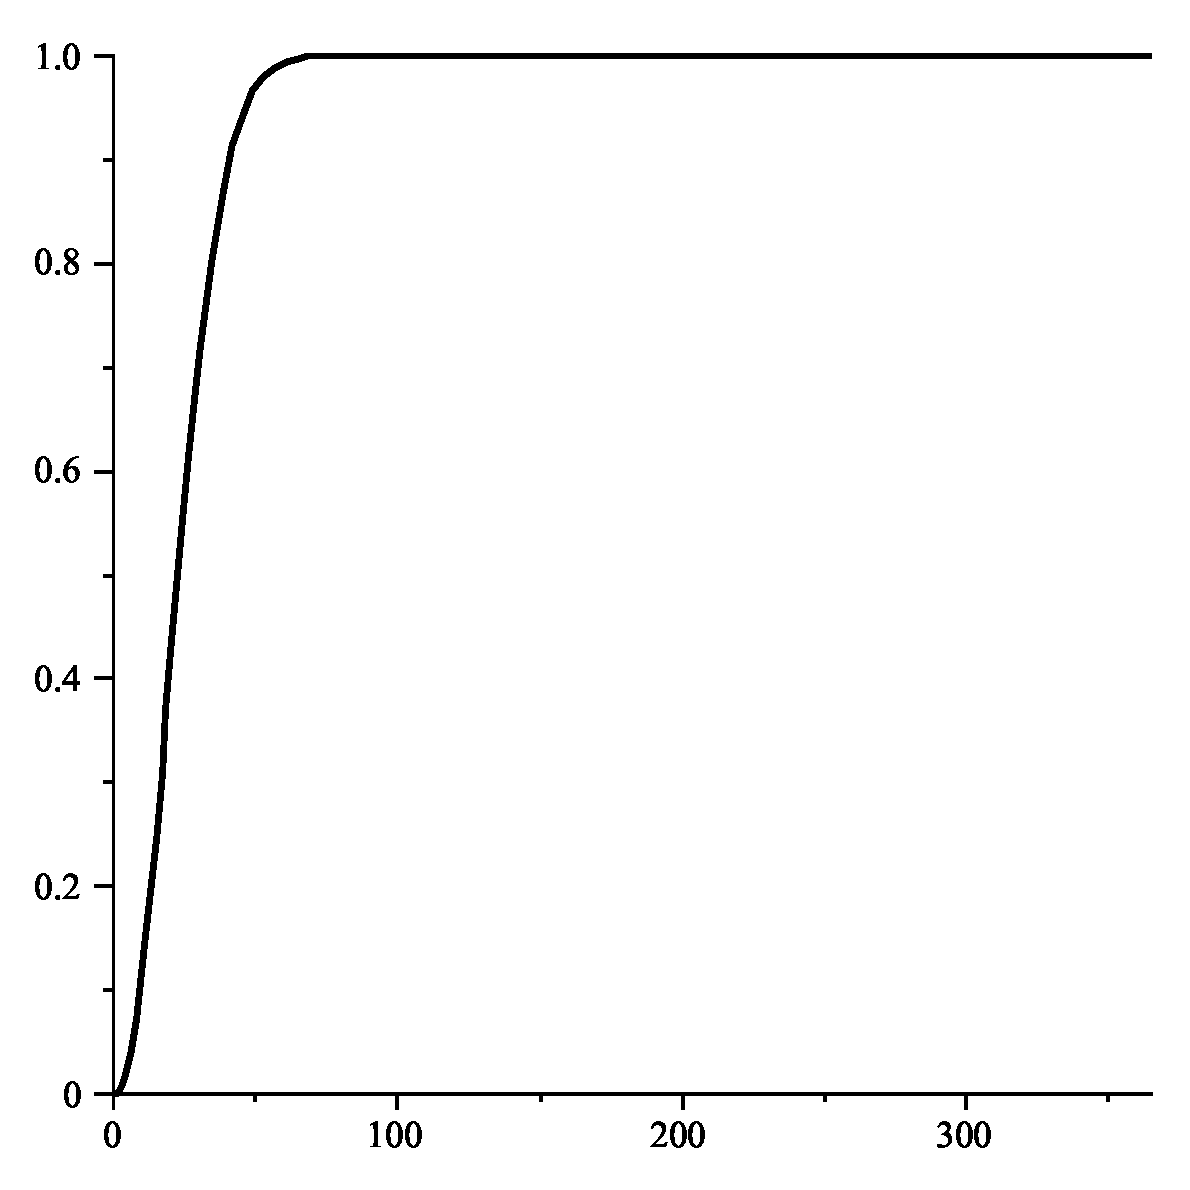
\includegraphics[width=6cm]{figs/birthday365.eps}
\end{center}
\caption{\label{fig:birthday} Birthday paradox: $\Pr_{365}(n)$.}
\end{figure}

When the load factor is much less than $1$, the average number of balls per bin
is small. If the load factor exceeds $1$ then the average number is large. In 
each case analysis is not too difficult. For hashing to be practical, we need 
to be able to fill a hash table as much as possible before we spend valuable 
time \defnfont{rehashing} --- that is, allocating more space for the table
 and reassigning hash codes via a new hash function. Thus we need to analyse 
 what happens when the load factor is comparable to $1$, that is, when the 
 number of balls is comparable to the number of bins. This also turns out to be
 the most interesting case mathematically.

\subsubsection{Theoretical analysis of hashing}

In addition to the basic operations for arrays, we also 
consider the computation of the hash address of an item to be an elementary 
operation.

Chaining is relatively simple to analyse. 

\begin{Lemma}\label{lem:sc}
The expected running time for unsuccessful search
in a hash table with load factor \(\lambda\) using
separate chaining is given by 
$$T_{\mathrm{us}}(\lambda)= 1+\lambda. $$
The expected running time for successful search is $O(1 + \lambda/2)$.

Update, retrieval, insertion and deletion all take time that is $O(1+\lambda)$.
\end{Lemma}
\begin{proof}
In an unsuccessful search for a key \(k\), the computation of
the hash address, \(h(k)\), takes one elementary
operation. The average running time to unsuccessfully search for the
key at that address is equal to the average length of the
associated chain, \(\lambda=\frac{n}{m}\). Thus in total
$T_{\mathrm{us}}(\lambda) = 1 + \lambda = 1 + n/m$.

The result for successful search and other operations 
now follows from Lemma~\ref{lem:ss-us}, since update, retrieval and deletion from a 
linked list take constant time.
\end{proof}

To analyse open addressing, we must make some extra assumptions. We use the 
\defnfont{uniform hashing hypothesis}: each configuration of $n$ keys in a 
hash table of size $m$ is equally likely to occur. This is what we would expect 
of a truly ``random" hash function, and it seems experimentally 
to be a good model for double hashing. Note that this is stronger than just 
requiring that each key is independently and uniformly likely to hash initially 
to each slot before collision resolution (``random balls in bins").
It also implies that all probe sequences are equally likely.

\begin{Lemma}\label{lem:oadh}
Assuming the uniform hashing hypothesis holds, 
the expected number of probes for search in a hash table satisfy
$$
T_{\mathrm{us}}(\lambda) \leq \frac{1}{1-\lambda} 
$$
and
$$ 
T_{\mathrm{ss}}(\lambda) \leq \frac{1}{\lambda} \ln \frac{1}{1-\lambda}.
$$
\end{Lemma}

\begin{proof} 
The average number of probes for an
unsuccessful search is
\(
T_{\mathrm{us}}(\lambda) = \sum_{i=1}^{n}i p_{m,n}(i)
\)
where \(p_{m,n}(i)\) denotes the probability of exactly \(i\)
probes during the search. Obviously, 
\(p_{m,n}(i) = \Pr (m,n,i) - \Pr (m,n,i+1)\) where 
\(\Pr (m,n,i)\) is the probability of \(i\) or more probes
in the search. By a similar argument to that used in the
birthday problem analysis we have for $i\geq 2$
$$
\Pr (m,n,i) = \frac{n}{m}\cdot \frac{n-1}{m-1} \cdots \frac{n-i+2}{m-i+2}
$$
while $\Pr (m,n,1) = 1$.
Note that clearly $\Pr (m,n,i) \leq (n/m)^{i-1} = \lambda^{i-1}.$
Thus
\begin{eqnarray*}
T_{\mathrm{us}}(\lambda) & = &
\sum\limits_{i=1}^{n}i\left ( 
{\textstyle \Pr (n,m,i) - \Pr (n,m,i+1) }\right ) \\
& \le &
\sum\limits_{i=1}^{\infty}i\left ( 
{\textstyle \Pr (n,m,i) - \Pr (n,m,i+1)}\right ) 
= \sum\limits_{i=1}^{\infty} \Pr (n,m,i) 
\le  
\sum\limits_{i=1}^{\infty} \lambda^{i-1} = \frac{1}{1-\lambda} = \frac{m}{m-n}.
\end{eqnarray*}

The result for successful search now follows by averaging. We have
\begin{align*}
T_{\mathrm{ss}}(\lambda) & \leq \frac{1}{n} \sum_{i=0}^{n-1} \frac{m}{m-i} \\
& = \frac{1}{\lambda} \sum_{j=m-n+1}^m \frac{1}{j}\\
& \leq \frac{1}{\lambda} \int_{n-m}^n dx/x = \frac{1}{\lambda} \ln\left(\frac{m}{m-n}\right) = \frac{1}{\lambda}
\ln\left(\frac{1}{1-\lambda}\right).
\end{align*}
\end{proof}

\begin{note}
It can be shown that the exact values are
\begin{align*}
T_{\mathrm{us}}(\lambda) & = \frac{m+1}{m-n+1} \approx \frac{1}{1-\lambda}\\
T_{\mathrm{ss}}(\lambda) & = \frac{m+1}{n} \left( H_{m+1} - H_{m-n+1} \right) 
\approx \frac{1}{\lambda} \ln\left(\frac{1}{1-\lambda}\right)
\end{align*}
so that the upper bounds in the theorem are asymptotically precise as $m\to \infty$.
\end{note}

Good implementations of OADH have been shown in theory and practice to be well 
described by the simple uniform hashing model above, so we may safely use the above
results. 

However, OALP is not well 
described by the uniform hashing model, because of its clustering 
behaviour. It can be analysed, however, in a similar but more complicated manner.

\begin{Lemma}\label{lem:oalp}Assuming uniformly hashed random input,
the expected number of probes for successful, $T_{\mathrm{ss}}(\lambda)$,
and unsuccessful, $T_{\mathrm{us}}(\lambda)$, search in a hash table using 
OALP are, respectively, 
\[
T_{\mathrm{ss}}(\lambda)\approx
0.5 \left ( 1 + \frac{1}{1-\lambda}\right ) 
\; \;\;\; 
\mathrm{and}
\; \;\;\; 
T_{\mathrm{us}}(\lambda)\approx
0.5 \left ( 1 + \left ( \frac{1}{1-\lambda} \right )^2 \right )
\]
\end{Lemma}
\begin{proof}
The proof is beyond the scope of this book (see Notes).
\end{proof}

The relationships in Lemma~\ref{lem:oalp} and Lemma~\ref{lem:oadh}
completely fail when \(\lambda=1\). But the latter situation indicates a full 
hash table, and we should avoid getting close to it anyway. 

Unlike OALP and OADH, the time estimates for separate chaining (SC) remain
valid with data removals. Because each chain may keep several 
table elements, the load factor may be more than $1$.

\begin{table}[htb!]
  \caption{\label{tbl-hash}Average search time bounds in hash tables with
           load factor $\lambda$.} 
 \centerline{
  \begin{tabular}{|c|ccc|ccc|} \hline
   \(\lambda\) & 
   \multicolumn{3}{c|}{Successful search: $T_{\mathrm{ss}}(\lambda)$} &
   \multicolumn{3}{c|}{Unsuccessful search: $T_{\mathrm{us}}(\lambda)$} 
   \\ \cline{2-7}
               & \textbf{SC} & \textbf{OALP} & \textbf{OADH} 
               & \textbf{SC} & \textbf{OALP} & \textbf{OADH}\\ \hline
0.10 & 1.05 & 1.06 & 1.05 & 1.10 & 1.12 & 1.11 \\
0.25 & 1.12 & 1.17 & 1.15 & 1.25 & 1.39 & 1.33 \\
0.50 & 1.25 & 1.50 & 1.39 & 1.50 & 2.50 & 2.0 \\
0.75 & 1.37 & 2.50 & 1.85 & 1.75 & 8.50 & 4.0 \\
0.90 & 1.45 & 5.50 & 2.56 & 1.90 & 50.5 & 10.0 \\
0.99 & 1.49 & 50.5 & 4.65 & 1.99 & 5000.0 & 100.0 \\ \hline
  \end{tabular}}
\end{table}

Table~\ref{tbl-hash} presents the above theoretical 
estimates of the search time in the OALP, OADH, and SC hash tables under 
different load factors. Average time measurements for actual hash
tables~\cite{standish} are close to the estimates for SC tables in  the whole
range \(\lambda \le 0.99\) and seem to be valid for larger
values of \(\lambda\), too. The measurements for OADH tables
remain also close to the estimates up to  \(\lambda = 0.99\).
But for OALP tables, the measured time is considerably
less than the estimates if \( \lambda > 0.90\) for a successful search and 
\( \lambda > 0.75\) for an unsuccessful search.

\begin{Example}
The expected performance of hashing depends only on the load factor.
If \(\lambda = 0.9\), OADH 
double hashing takes on the average 2.56 and 10 probes for 
successful and unsuccessful search, respectively. But 
if \(\lambda = 0.5\), that is, the same keys are stored 
in a roughly twice larger table, the same numbers decrease
to 1.39 and 2 probes.
\end{Example}


\subsection{Implementation of hashing}

\subsubsection{Resizing} 
One problem with open addressing is that successive insertions may cause the table
to become almost full, which degrades performance. Eventually we will need to 
increase the table size. Doing this each time an element is inserted is very 
inefficient. It is better to use an upper bound, say $0.75$, on the load factor, 
and to double the array size when this threshold is exceeded. This will then require 
recomputing the addresses of each element using a new hash function.

The total time required to resize, when growing a table from $0$ to $m=2^k$ elements,
is of order $1 + 2 + 4 + 8 + \dots + 2^{k-1} = 2^k - 1 = m - 1$. Since the $m$ 
insertions take time of order $m$ (recall the table always has load factor 
bounded away from $1$), the average insertion time is still $\Theta(1)$.

\subsubsection{Deletion}

It is quite easy to delete a table entry from a hash table with separate 
chaining (by mere node deletion from a linked list). However, open addressing 
encounters difficulties. If a particular table entry is physically removed
from a OA-hash table leaving an empty entry in that place, the search for 
subsequent keys becomes invalid. This is because the OA-search terminates when 
the probe sequence encounters an empty table entry. Thus if a previously occupied 
entry is emptied, all probe sequences that 
previously travelled through that entry will
now terminate before reaching the right location. 

To avoid this problem, the deleted entry is normally marked in such a way that
insertion and search operations can treat it as an empty and 
nonempty location, respectively. Unfortunately, such a policy results in hash 
tables packed with entries which are marked as deleted. But in this case the 
table entries can be rehashed to preserve only actual data and really delete all
marked entries. In any case, the time to delete a table entry remains \(O(1)\) 
both for SC  and OA hash tables.

\subsubsection{Choosing a hash function}
\label{sec:choice:hash:fun} 

Ideally, the hash 
function, \(h(k)\), has to map keys uniformly and randomly onto 
the entire range of hash table addresses. Therefore, the
choice of this function has much in common with the choice of
a generator of uniformly distributed pseudorandom numbers. 
A randomly chosen key \(k\) has to equiprobably hash to each
address so that uniformly distributed keys produce uniformly
distributed indices \(h(k)\). A poorly designed hash function
distributes table addresses nonuniformly and tends to
cluster indices for contiguous clusters of keys. 
A well designed function scatters the keys as to avoid
their clustering as much as possible.

If a set of keys is fixed, there always exists a \defnfont{perfect hash function}
that maps the set one-to-one onto a set of table indices and thus entirely 
excludes collisions. However, the problem is how to design such a function as
it should be computed quickly but without using large tables.
There exist techniques to design perfect hash functions for given sets of keys. 
But perfect hashing is of very limited interest because in most applications 
data sets are not static and the sets of keys cannot be pre-determined.

Four basic methods for choosing a hash function
are \defnfont{division}, \defnfont{folding}, \defnfont{middle-squaring}, and 
\defnfont{truncation}.
\begin{description}
\item[Division] assuming the table size is a prime number \(m\) 
and keys, \(k\), are integers,
the quotient, \(q(k,m)=\left \lfloor \frac{k}{m} \right \rfloor \), 
and the remainder, \(r(k,m)=k \mod m\), of the integer division of
\(k\) by \(m\) specify the
probe decrement for double hashing and the value
of the hash function \(h(k)\), respectively:
$$
h(k) = r(k,m) \mbox{ and }
\Delta(k) = \max \left \{
1, \ q(k,m) \bmod m \right\} \quad . 
$$
The probe decrement is put to the range \([1,\ldots,m-1]\) because all
decrements should be nonzero and point to the indices
\([0,1,\ldots,m-1]\) of the table. The reason that $m$ should be prime is that 
otherwise some slots may be unreachable by a probe sequence: for example if 
$m=12$ and $\Delta(k) = 16$, only $3$ slots will be probed before the sequence
returns to the starting position.

\item[Folding] an integer key \(k\) is divided into sections and 
the value \(h(k)\) combines sums, differences, and products of
the sections (for example, a 9-digit decimal key, such as 
\(k=013402122\), can be split into three sections:
013, 402, and 122, to be added together for getting 
the value \(h(k)=537\) in the range \([0,\ldots,2997]\)).

\item[Middle-squaring] a middle section of an integer key
\(k\), is selected and squared, then a middle section of 
the result is the value \(h(k)\) (for example, the squared middle section, 402, of 
the above 9-digit key, \(k=013402122\), results in 161604, and
the middle four digits give the value \(h(k)=6160\) in the range
\([0,\ldots,9999]\)).

\item[Truncation] parts of a key are simply cut out and 
the remaining digits, or bits, or characters are used
as the value \(h(k)\)  
(for example, deletion of all but last three digits 
in the above 9-digit key, \(k=013402122\),
gives  
the value \(h(k)=122\) in the range \([0,\ldots,999]\)).
While truncation is extremely fast, the keys do not scatter
randomly and uniformly over the hash table indices. This is
why truncation is used together with other methods, but 
rarely by itself.
\end{description}

Many real-world hash functions combine some of the above methods.
                                            
We conclude by discussing the idea of \emph{universal hashing}. We have seen 
(in the section on quicksort) the idea of using randomization to 
protect against bad worst-case behaviour. An analogous idea works for hashing.
                                           
If a hash table is dynamically changing and its elements 
are not known in advance, any fixed hash function can result in 
very poor performance on certain inputs, because of collisions. 
Universal hashing allows us to reduce the probability of this occurrence
by randomly selecting the hash function at run time from a large set
of such functions. Each selected function still may be bad for a
particular input, but with a low probability
which remains equally low if the same input is met once again.
Due to its internal randomisation, universal hashing behaves well even for
totally nonrandom inputs. 

\begin{Definition}
Let \(K\), \(m\), and \(F\) denote
a set of keys, a size of a hash table (the range of indices),
and a set of hash functions mapping \(K\) to \(\{0,\ldots,m-1\}\),
respectively. Then \(F\) is a \defnfont{universal class} if any
distinct pair of keys \(k,\kappa \in {K}\)  collide
for no more than \(\frac{1}{m}\) of the functions in the class \({F}\),
that is,
\[
\frac{1}{|{F}|}
\left| \raisebox{10pt}{} \left\{ h \in {F} \mid \ h(k) = h(\kappa)\right\}\right|
\le \frac{1}{m} \quad .
\]
%where \(|Z|\) denotes cardinality of a finite
%set \({Z}\).

\end{Definition}
Thus in the universal class all key pairs behave well and the
random selection of a function from the class results in a probability of at most
\(\frac{1}{m}\) that any pair collide.

One popular universal class of hashing functions is produced by
a simple division method. It assumes the keys are integers and
cardinality of
the set of keys \({K}\) is a prime number larger 
than the largest actual key. The size \(m\) of the hash
table can be arbitrary. This universal class is described by
the next theorem.

\begin{Theorem}[Universal Class of Hash Functions] 
\label{the:ucf}
Let \({K}=\{0,\ldots,p-1\}\) and \(|{K}| = p\) be
a prime number. 
For any pair of integers \(a \in \{1, \ldots, p-1\}\)
and \(b \in \{0, \ldots, p-1\}\), let
\(
h_{a,b}(k) = \left ( (ak + b) \bmod p \right ) \bmod m
\).
Then
\[
{F} = \{h_{a,b} \mid \ 1 \le a < p \;\; \mathrm{and} \;\; 0 \le b < p \}
\]
is a universal class.
\end{Theorem}
\begin{proof}
It is easily shown that the number of collisions in the
class \({F}\), 
\[
\left| \raisebox{10pt}{} \{h\in {F} \mid  h(k)= h(\kappa); \ k,\kappa\in {K}\}\right|,
\]
is the number of distinct numbers \((x,y)\);
\(0 \le x,y < p\) such that 
\(x \bmod m = y \bmod m\). Let us denote the latter property: 
\(x \equiv y \pmod m\). %; (\hspace*{-3mm}\mod n)\).
It is evident that \(h_{a,b}(k) = h_{a,b}(\kappa)\) iff 
\[
(ak + b ) \bmod p  \equiv 
(a\kappa + b ) \bmod p  \pmod m \quad .
\]

Then for any fixed \(k, \kappa < p\), there is one-to-one
correspondence between the pairs \((a,b)\) such that
\(0 < a < p\) and \(0 < b < p\) and \(h_{a,b}(k) = h_{a,b}(\kappa)\),
and the pairs of distinct numbers \((x,y)\) with the
property that \(0 \le x,y < p\) and \(x \equiv y \pmod n\).
The correspondence is given in one direction by
\[
x = (ak + b) \bmod p; \;\; y = (a\kappa + b) \bmod p
\]
where \(x \ne y\) since 
\[
\{ az + b \mid \ z = 0, \ldots, p-1\} = \{0, \ldots, p-1\}
\]
when \(p\) is prime and \(a \ne 0\). In the other direction
the correspondence is given by the condition that \(a\) and
\(b\) are the unique integers in \(\{0, \ldots, p-1\}\) such
that
\[
ak + b \equiv x \pmod p \; \;\;\mathrm{and}\;\;\;
a\kappa + b \equiv y \pmod p \quad .
\]
These equations have a unique solution for \(a\) and \(b\)
since \(p\) is prime, and \(a \ne 0\) since \(x \ne y\).

Clearly \(|{F}| = p(p-1)\). Now let us find out how many 
pairs of distinct numbers
\((x,y)\) exist such that \(0 \le x,y < p\) and 
\(x \equiv y \pmod m\). For any fixed \(s < m\) there are
at most \( \left \lceil \frac{p}{m} \right \rceil \) numbers
\(x < p\) such that \(x \equiv s \pmod m\). Since \(p\) and
\(m\) are integers,
\(
\left \lceil \frac{p}{m} \right \rceil \le \frac{p-1}{m} +1
\).
Therefore for each \(x < p\) there are no more than
\(\frac{p}{m} -1 \le \frac{p-1}{m}\) numbers \(y < p\)
distinct from \(x\) such that \(x \equiv y \pmod m\), and
the total number of such pairs \((x,y)\) is at most 
\(\frac{p(p-1)}{m}\). Hence for any fixed distinct
pair of keys \((k,\kappa)\) the fraction of \({F}\)
that cause \(k\) and \(\kappa\) to collide is at
most \(\frac{1}{m}\), so the class \({F}\) is universal.
\end{proof}

This suggests the following strategy for 
choosing a hash function at run time: (i) find 
the current size of the set of keys to hash; 
(ii) select the next 
prime number \(p\) larger than the size of the key set found;
({iii}) randomly choose integers \(a\) and \(b\)
such that \(0 < a < p\) and \(0 \le b < p\), and 
({iv}) use the function \(h_{a,b}\) 
defined in Theorem~\ref{the:ucf}.


\subsection*{Exercises}

\begin{Exercise}\label{exr:java:hash}
The Java programming language (as of time of writing)
uses the following hash function $h$ for character strings. 
Each character has a Unicode value represented by an integer (for example, the 
upper case letters $A, B, \dots, Z$ correspond to $65, 66, \dots, 90$ and the 
lower case $a, b, \dots, z$ correspond to $97, 98, \dots, 122$). Then 
$h$ is computed using 32-bit integer addition via
$$h(s) = s[0]*31^{n-1} + s[1]*31^{n-2} + \dots + s[n-1]*31 + s[n].$$

Find two 2-letter strings that have the same hash value. How could you use this 
to make $2^{100}$ different strings all of which have the same hash code?
\end{Exercise}

\begin{Exercise}\label{exr:hash:oalp}
Place the sequence of keys \(k=10, 26, 52, 76, 13, 8, 3, 33, 60, 42\) 
into a hash table of size 13 using the modulo-based hash address \(i = k \mod 13\) 
and linear probing to resolve collisions.
\end{Exercise}

\begin{Exercise}\label{exr:hash:oadh}

Place the sequence of keys \(k=10, 26, 52, 76, 13, 8, 3, 33, 60, 42\) 
into a hash table of size 13 using the modulo-based hash address \(i = k \mod 13\) 
and double hashing with the secondary hash function 
\(\Delta(k)=\max\{1, k/13 \}\) to resolve collisions.
\end{Exercise}

\begin{Exercise}\label{exr:hash:sc}
Place the sequence of keys \(k=10, 26, 52, 76, 13, 8, 3, 33, 60, 42\) 
into a hash table of size 13 using separate chaining to resolve collisions.
\end{Exercise}


\section{Notes}

Binary search, while apparently simple, is notoriously hard to program 
correctly even for professional programmers: see \cite{bentley-prog-pearls} 
for details.

The expected height of a randomly grown BST was shown to be $\Theta(\log n)$ by 
J. M. Robson in 1979. After much work by many authors 
it is now known that the average value is 
tightly concentrated around $\alpha \ln n$ where $\alpha$ is the root of 
$x \ln (2e/x) = 1$, $\alpha \cong 4.311$.  

The historically first balanced binary search tree was
proposed in 1962 by G. M. Adelson-Velskii and E. M. Landis, hence the 
name AVL tree. Red-black trees were developed in 1972 by R. Bayer under the 
name ``symmetric binary B-trees" and received their present name and definition 
from L. Guibas and R. Sedgewick in 1978. AA-trees were proposed by A. Anderson 
in 1993.

Multiway B-trees were proposed in 1972 by R. Bayer and E. McCreight. 

According to D. Knuth, hashing was invented at IBM in early 1950's 
simultaneously and independently by H. P. Luhn (hash tables with SC) and 
G. M. Amdahl (OALP). 

The analysis of OALP hashing was first performed by D. Knuth in 1962. This was 
the beginning of the modern research field of analysis of algorithms.

The random balls in bins model can be analysed in detail by more advanced methods
than we present in this book (see for example \cite{flaj-sedg}). Some natural questions are
\begin{itemize}
\item When do we expect all bins to have at least one ball?
\item What proportion of boxes are expected to be empty when $n \approx m$?
\item What is the expected maximum number of balls in a box when $n \approx m$?
\end{itemize}
The answers are applicable to our analysis of chaining: when are all chains 
expected to be nonempty? how many chains are empty when the average chain 
length is $\Theta(1)$? what is the maximum chain length when the average chain
length is $\Theta(1)$? The answers are known to be, respectively: when 
$n \approx m \ln m$; about $e^{-\lambda}$; $\Theta(\log n/\log \log n)$. The last
result is much harder to derive than the other two.  
